% 1 страница 
\newpage
\sodef\so{}{.3em}{.75em}{.55em}
\pagecolor[cmyk]{0,0,0.13,0}
\setcounter{page}{6}
\pagestyle{fancy}
\fancyhf{}
\fancyfoot[L]{\thepage}
\begin{minipage}[t]{0.4\textwidth}
\setlength{\parindent}{4ex}
\subsection*{Приложение}
\hspace{4ex}Перейдём теперь ко второй части нашего рассказа, из которой наиболее настойчивые читатели узнают доказательство гипотезы Эйлера.
\par
30 марта 1796 года девятнадцатилетний Гаусс доказал возможность построения правильного семнадцатиугольника циркулем и линейкой. С этого дня начинается дневник Гаусса -- летопись его удивительных открытий. Вторая запись в дневнике появилась уже 8 апреля. В ней сообщалось, что найдено строгое доказательство <<золотой>> теоремы -- так назвал Гаусс гипотезу Эйлера. Он переоткрыл её, ещё учась в брауншвейгской гимназии, когда ему не были доступны произведения Эйлера, Лагранжа, Лежандра, с которыми он познакомился лишь после переезда в Геттинген в 1795 году. Вначале он, как и его предшественники, замечает утверждение для \textit{a}=$-$1, затем, уже угадав результат для общего случая, последовательно разбирает случай за случаем, продвинувшись дальше других: им рассмотрены \textit{a}=$\pm$2, $\pm$3, $\pm$5, $\pm$7. Наконец, 8 апреля 1796 года он находит общее доказательство, которое Кронекер (1823 -- 1891) очень метко назвал <<пробой сил гауссова гения>>. Доказательство проводится двойной индукцией по \textit{a} и \textit{p}; Гауссу приходится придумывать существенно различные соображения для рассмотрения восьми (!) различных случаев. Нужно было иметь не только поразительную изобретательность, но и удивительное мужество, чтобы не остановиться на этом пути. Позднее Гаусс нашёл ещё шесть доказательств <<золотой>> теоремы (ныне их известно около пятидесяти). Как это часто бывает, после того как теорема доказана, удаётся найти доказательства много более простые, чем первоначальное. Мы приведём здесь доказательство, мало отличающееся от третьего доказательства Гаусса. В его основе лежит ключевая лемма, доказанная Гауссом не ранее 1808 года.
\\
\par
\large{\so{Лемма 2}. Пусть \textit{p = $2$k $+$ $1$ --- простое число, а --- целое число, 0 $< |a| \leq 2k;$ $r_1, r_2, \ldots, r_k$ --- вычеты чисел $a, 2a, \ldots, ka;$ $\nu$ --- число отрицательных среди них.}}
\end{minipage}
\hspace{1.25cm}
\begin{minipage}[t]{0.4\textwidth}
\setlength{\parindent}{4ex}
\large{\textit{Тогда}
\\
\\
$$a^k \equiv (-1)^{\nu}(mod \,\textit{p}) \eqno{(6)}$$
\\ 
\par
Применяя критериий Эйлера, получаем такое следствие:
\par
\so{Критерий квадратичности вычета}. \textit{Вычет является квадратичным тогда и только тогда, когда фигурирующее в лемме $2$ число $\nu$ чётно.}
\par
\so{Доказательство леммы 2}. Заметим, что все вычеты \textit{$r_1, \ldots, r_k$} различны по абсолютной величине. Это следует из того, что сумма и разность любых двух из них не делится на \textit{p: $r_i \pm r_j \approx (i \pm j)a, i \neq j; |i \pm j| < p.$} Таким образом, набор модулей |$r_1$|, \ldots, |$r_k$| --- это числа 1, 2, \ldots, \textit{k}, в некотором порядке. В результате произведение \textit{a $\cdot$} 2\textit{a\ldots ka = $a^{k}$k!} при делении на \textit{p} даёт тот же остаток, что \textit{$r_1, \ldots, r_k = (-1)^{\nu}k!.$} Учитывая, что \textit{k!} не делитсчя на простое число \textit{p}, получаем (6).
\par
\so{Доказательство гипотезы Эйлера}. Заметим, что в приводимом ниже рассуждении уже не используется простота \textit{p} --- она в полной мере использована в лемме Гаусса. Отметим на числовой оси точки (рис. 1, \textit{а, б) m$\frac{p}{2}$}, если \textit{a}<0; \textit{m} = 0, 1, 2, \ldots, |\textit{a}| --- синие точки (\textit{m} --- их номера). Занумеруем интервалы с концами в этих точках по номерам левых концов (на рисунках номера интервалов --- красные). Отметим теперь \textit{a, 2a, \ldots, ka} --- зелёные точки; так как \textit{a} --- целое, не делящееся на \textit{p}, то синие точки не могут сопасть}
\end{minipage}


\begin{figure}[h]
\begin{flushleft}
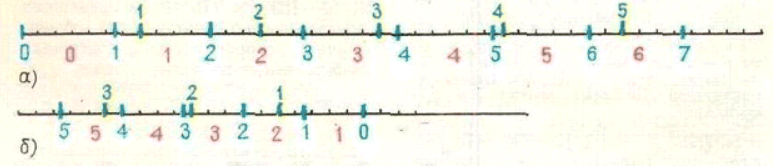
\includegraphics[width = 19cm]{picture1}
\caption*{\hspace*{3ex}Рис.1, a. На рисунке \textit{p} = 11 (\textit{k = 5}), \textit{a} = 7, \textit{$\nu$} = 3.
\\\hspace{3ex}Рис. 1, б. На рисунке \textit{p} = 7 (k = 3), \textit{a} = -5, \textit{$\nu$} = 2.}
\end{flushleft}
\end{figure}
% конец 1 страницы

% 2 страница
\newpage
\pagestyle{fancy}
\fancyhf{}
\fancyfoot[R]{\thepage}
\begin{figure}[h]
\begin{flushleft}
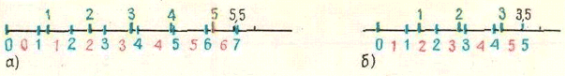
\includegraphics[width = 19cm]{picture2}
\end{flushleft}
\caption*{\hspace{0.5cm}Рис. 2.}
\end{figure}

\begin{minipage}[t]{0.4\textwidth}
\large{с зелёными, причём все зелёные точки попадут в какие-то из построенных интервалов $\left(|\textit{a}\frac{\textit{p}}{2} > |\textit{a}|\textit{k}\right)$. Легко заметить, что фигурирующее в лемме число $\nu$ --- это число зелёных точек, попавших в интервалы с нечётными номерами (докажите!).
\setlength{\parindent}{4ex}

Подвергнем теперь нашу картинку преобразованию подобия с коэффициентом $\frac{1}{a}$ (рис. 1 перейдёт в рис. 2). При этом синие точки перейдут в точки, делящие отрезок $\left[0, \frac{p}{2} \right]$ на |\textit{a}| равных частей, а зелёные точки --- в целочисленные точки 1, 2, \ldots, \textit{k}.

Нумерация интервалов теперь будет зависеть от знака \textit{a}: при \textit{a} > 0 они нумеруются номерами левых концов, при \textit{a} < 0 --- номерами правых концов; $\nu$ --- число целочисленных точек в интервалах с нечётными номерами. Если мы увеличим \textit{p} на 4\textit{al}, то в каждый интервал добавится точно 2\textit{l} целых точек. Это следует из того, что при сдвиге интервала на целое число количество целых точек в нём не меняется, а на любом отрезке целочисленной длины \textit{n} с нецелочисленными концами имеется ровно \textit{n} целых точек (докажите!). Итак, при изменении \textit{p} на \textit{p} + 4\textit{al} величина $\nu$ изменится на чётное число, а $(-1)^{\nu}$ не изменрится.  Значит, для всех \textit{p} в арифметической прогрессии $p = 4aq + r$  значение $(-1)^{\nu}$ --- одно и то же, и гипотеза Эйлера доказана.

Одновременно указан некоторый способ выяснить, является ли $a$ квадратичным}
\end{minipage}
\hspace{1.25cm}
\begin{minipage}[t]{0.4\textwidth}
\large{вычетом для $p$. Нужно взят остаток $r$ от деления $p$ на 4$a$ (для удобства положительный); разделить $\left(\,0,\, \frac{r}{2}\,\right)$ на |$a$| частей, занумеровав их номерами левых (правых) концов, если $а$ --- положительное (отрицательное); сосчитать число $\nu$ целых точек, попавших в интервалы с нечётными номерами; a --- квадратичный вычет в том и только том случае, когда $\nu$ чётно.
\setlength{\parindent}{4ex}

Проделаем эти вычисления для $a$ = 2, чтобы подтвердить наблюдения Эйлера, о которых говорилось на стр. 5. Пусть $a$ = 2; Тогда достаточно рассмотреть $r$ = 1, 3, 5, 7, поскольку в остальных случаях арифметическая прогрессия не будет содержать простых чисел. Как видно из рис. 3, число 2 является квадратичным вычетом для $$p = 8q +1, p = 8q + 7,$$
то есть $p = 8q \pm 1.$}
\\
\\
\hspace*{1ex}
\small{У\,п\,р\,а\,ж\,н\,е\,н\,и\,е. Покажите, что -2 есть квадратичный вычет для $p = 8q + 1, p = 8q + 3.$}
\par
\hspace{4ex}\large{Аналогично рассматривается случай $a$ = $\pm$3. Приведём итоги вычислений (таблица для $\nu$):}\\\\ 
\renewcommand{\arraystretch}{1.4}
\begin{tabular}{p{0.15\textwidth}||*{3}{p{0.15\textwidth}|}p{0.15\textwidth}}
\hline
\diagbox[width = 0.2\textwidth]{$a$}{$r$} & \makecell{1} & \makecell{5} & \makecell{7} & \makecell{11}\\
\hline\hline
\rule{0cm}{0.7cm}
\makecell{3} & \makecell{0} & \makecell{1} & \makecell{1} & \makecell{2}\\
\hline
\rule{0cm}{0.7cm}
\makecell{-3} & \makecell{0} & \makecell{1} & \makecell{2} & \makecell{3}\\
\hline
\end{tabular}
\end{minipage}
\begin{figure}[h]
\begin{flushleft}
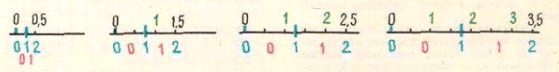
\includegraphics[width = 19cm]{picture3}
\end{flushleft} 
\caption*{\hspace*{0.5cm}Рис. 3. $r$ = 1, $a$ = 2, $\nu$ = 0; $r$ = 3, $a$ = 2, $\nu$ = 1; $r$ = 5, $a$ = 2, $\nu$ = 1; $r$ = 7, $a$ = 2, $\nu = 2$.}
\end{figure}\\
% конец 2 страницы